\clearpage
\section{Fixed points and stability}
\begin{colbox}
	\begin{enumerate}
		\item Consider the system \(\dot{x}=\tan x\) restricted to the segment \(x \in \ins{-\pi/2,\pi/2}\). Find and classify the fixed points in this segment.
		\item Consider the system \(\dot{x} = \ins{1-e^{-x^2}}\ins{1-x}\) \begin{enumerate}
			\item Find and classify the fixed points of the system using linear stability analysis. If linear stability analysis fails determine stability using a graphical method instead.
			\item For an iitial condition very close to the stable fixed point, find how \(x(t)\) behaves at long times.
		\end{enumerate}
		\item Consider the system \(\dot{x}=-x^3\)\begin{enumerate}
			\item Find and classify the fixed points of the system
			\item Solve this equation exactly for a general initial condition and describe how \(x(t)\) behaves at long times. Compare with the long-time behavior you found. What is qualitatively differnent and why?
		\end{enumerate}
	\end{enumerate}
\end{colbox}
\subsection{tanx}
The fixed points can be found by solving
\begin{equation}
	\tan x = 0 \implies x=k\pi \quad k\in\mathbb{Z}
\end{equation}
therefore the only fixed point in the segment is (0,0), and it is unstable.
\subsection{Gaussian and linear}
\subsubsection{Fixed Points}
To begin the process we find points where we suspect there may be fixed points. From the form of the equation we can immediately tell that \(x=0,1\) are fixed points which we will investigate. To perform linear stability analysis we expand \(f\) in a taylor series around those points. First we derive
\begin{wrapfigure}{r}{0.3\textwidth}
	\begin{center}
		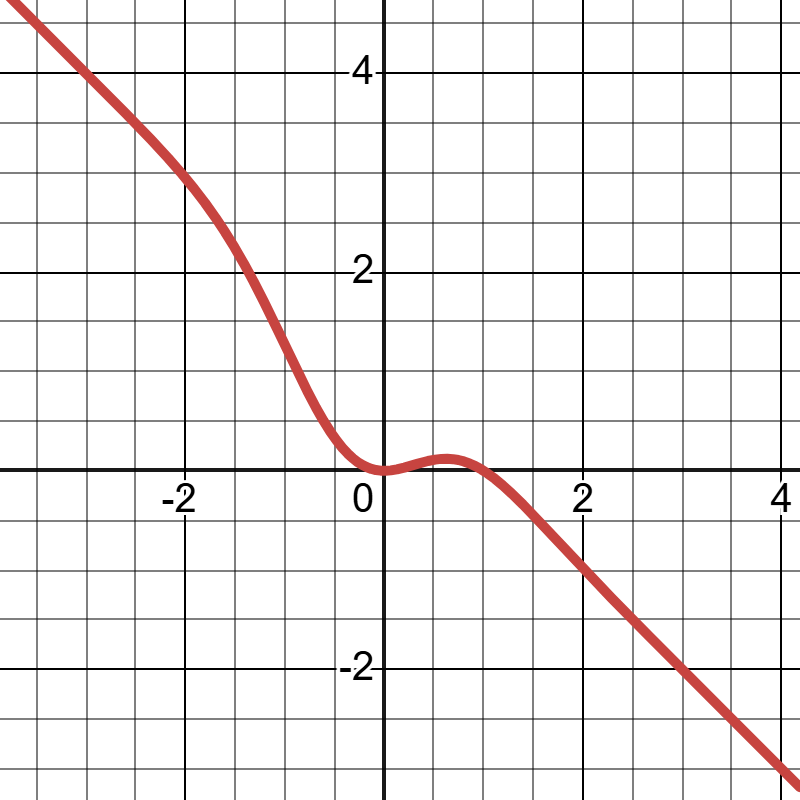
\includegraphics[width=0.3\textwidth]{desmos-graph.png}
	\end{center}
\end{wrapfigure}
\begin{align}
	f'(x) = \ins{2xe^{-x^2}}\ins{1-x}-1+e^{-x^2} = \begin{cases}
		0 & x=0\\
		\frac{1}{e}-1 & x=1
	\end{cases}
\end{align}
Therefore the point \(x=1\) is stable, and the point \(x=0\) requires a graphical analysis. Looking at the graph of the function we can see that at the point \(x=0\) going to the negative gives positive values for \(\dot{x}\), which stabilizes the point, but going to positive values also gives positive \(\dot{x}\), which pushes us away from the point, so \(x=0\) is not stable.
\subsubsection{Behavior at long times}
The stable point as we found is (1,0). We'll look at small perturbations around that point:
\begin{equation}
	x(t) = 1+\eta(t)
\end{equation}
therefore to first order
\begin{equation}
	\dot{\eta}=f'(1)\eta
\end{equation}
plugging the derivative in
\begin{equation}
	\dot{\eta} = \ins{\frac{1}{e}-1}\eta
\end{equation}
which is a simple ODE giving
\begin{equation}
	\eta = \eta_0 e^{\ins{\frac{1}{e}-1}t}
\end{equation}
so at long times its decays exponentially.
\subsection{third power}
\subsubsection{Fixed Points}
The right hand side obviously only has the real root \(x=0\) therefore that is the fixed point. As for stability
\begin{equation}
	f'(x) = -3x^2
\end{equation}
which is 0 at \(x=0\) so the test fails. Looking at the derivative around the point we see it's negative when \(x>0\) and positive when \(x<0\), therefore the point is stable.
\subsubsection{Exact solution}
the equation is
\begin{equation}
	\dot{x} = -x^3
\end{equation}
using separation of variables
\begin{equation}
	x^{-3}\dd{x} = -\dd{t}
\end{equation}
integrating
\begin{equation}
	\frac{1}{2}x^{-2} = t + C
\end{equation}
rearranging
\begin{equation}
	x = \ins{2\ins{t+C}}^{-0.5}
\end{equation}
using the initial condition
\begin{equation}
	x = \ins{2\ins{t+\frac{x_0^{-2}}{2}}}^{-0.5} = \frac{1}{\sqrt{2t+\frac{1}{x_0^2}}}
\end{equation}
simplifying
\begin{equation}
	x(t) = \frac{x_0}{\sqrt{2x_0^2 t + 1}}
\end{equation}
\subsubsection{Behavior at long times}
at long times the initial condition becomes small enough that we can write
\begin{equation}
	x(t) = \frac{x_0}{\sqrt{2x_0^2 t + 1}} \simeq \frac{x_0}{\abs{x_0}\sqrt{2t}} = \frac{sgn(x_0)}{\sqrt{2t}}
\end{equation}
so \(x\rightarrow 0\). This is similar to 2b in that it also goes to zero, but in 2b it decays exponentially while here it decays with the root of the time, which is much slower.